%tdepps stuff
\chapter{Time-Dependent Stacking Software Approach} \label{sec:tdepps}

As already indicated in chapter \ref{sec:csky_time_dep}, a different likelihood must be used to calculate time-dependent stacking.
The test statistic shown in chapter \ref{sec:theory} benefits from the fact that each event is independent of each other and thus PDF ratios can be used directly to calculate the likelihood ratio.
This also benefits the computational capacity.
If, on the other hand, there are several events in the same time window from different sources, these are counted several times and the background is also overestimated.
For a correct calculation, the original test statistic derived in \eqref{eq:TS_general}, which is again shown in equation \eqref{eq:general_ts}, must be considered,
\begin{equation}
    -2\ln{\hat{\Lambda}} = -2\sum_{k=1}^{N_{\text{srcs}}}\hat{\lambda}_{k,S} + 2\sum_{i=1}^{N_{evts}}\ln{\left(\frac{\sum_{k=1}^{N_{\text{srcs}}}\hat{\lambda}_{k,S}S_{i,k}}{\sum_{k=1}^{N_{\text{srcs}}}\langle\lambda_{k,B}\rangle B_{i,k}}+1\right)} \label{eq:general_ts}, \\
\end{equation}
with the expected values for the number of background events $\langle\lambda_{k,B}\rangle$ and signal events  $\hat{\lambda}_{k,S}$ and the PDFs for background $B$ and signal $S$ dependent on the source $k$ and event $i$.
The diagram in figure \ref{fig:new_method} illustrates the problem and the approach to solving it.

\begin{figure}
  \centering
  \scalebox{0.8}{
  \begin{tikzpicture}[scale=1]
    %\node at (2,-6) {\includegraphics[width=10cm]{images/bg_hist_and_contour.pdf}};
    % Koordinatensystem
    \draw[line width=0.25mm, ->] (-5,0) -- (-5,5);
    \draw[line width=0.25mm, ->] (-5,0) -- (10,0);
    \node at (10,-0.5) {time};
    \node at (-5.5,3) {rate};
    % Quellen
    \draw[line width=0.5mm, green] (-1,-1) -- (-1,4);
    \fill[pattern = north east lines, pattern color = green, opacity = 0.5,domain=-3:1,variable=\x]
    (-3,0)
    -- plot ({\x},{3.5})
    -- (1,0)
    -- cycle;
    \fill[pattern = north east lines, pattern color = green, opacity = 0.5,domain=-3:1,variable=\x]
    (-3,0)
    -- plot ({\x},{-0.5})
    -- (1,0)
    -- cycle;
    \draw[green] (-3,-0.5) -- (1,-0.5);
    \draw[green] (-3,3.5) -- (1,3.5);
    \draw[green] (-3,-0.5) -- (-3,3.5);
    \draw[green] (1,-0.5) -- (1,3.5);
    \node[green] at (-1,4.5) {$k=1$};

    \draw[line width=0.5mm, red] (2.5,-1) -- (2.5,4);
    \fill[pattern = north west lines, pattern color = red, opacity = 0.5,domain=0.5:4.5,variable=\x]
    (0.5,0)
    -- plot ({\x},{3.5})
    -- (4.5,0)
    -- cycle;
    \fill[pattern = north west lines, pattern color = red, opacity = 0.5,domain=0.5:4.5,variable=\x]
    (0.5,0)
    -- plot ({\x},{-0.5})
    -- (4.5,0)
    -- cycle;
    \draw[red] (0.5,-0.5) -- (4.5,-0.5);
    \draw[red] (0.5,3.5) -- (4.5,3.5);
    \draw[red] (0.5,-0.5) -- (0.5,3.5);
    \draw[red] (4.5,-0.5) -- (4.5,3.5);
    \node[red] at (2.5,4.5) {$k=2$};

    \draw[line width=0.5mm, blue] (6,-1) -- (6,4);
    \fill[pattern = north east lines, pattern color = blue, opacity = 0.5, domain=4:8,variable=\x]
    (4,0)
    -- plot ({\x},{3.5})
    -- (8,0)
    -- cycle;
    \fill[pattern = north east lines, pattern color = blue, opacity = 0.5,domain=4:8,variable=\x]
    (4,0)
    -- plot ({\x},{-0.5})
    -- (8,0)
    -- cycle;
    \draw[blue] (4,-0.5) -- (8,-0.5);
    \draw[blue] (4,3.5) -- (8,3.5);
    \draw[blue] (4,-0.5) -- (4,3.5);
    \draw[blue] (8,-0.5) -- (8,3.5);
    \node[blue] at (6,4.5) {$k=3$};
    % Samples
    %\draw[line width=0.5mm] (6,-2) -- (6,5);
    %\draw[line width=0.5mm] (0,-2) -- (0,5);
    %\node at (-3,5) {j=1};
    %\node at (3,5) {j=2};
    %\node at (8,5) {j=3};
    % Events
    %\draw[line width=0.5mm,orange] (5,-2) -- (5,1);
    %\draw[line width=0.5mm,orange] (8,-2) -- (8,1);
    %\draw[line width=0.5mm,orange] (3,-2) -- (3,1);
    \draw[line width=0.5mm,orange] (0.75,-1) -- (0.75,1);
    %\node at (0.9,-1.5) {\quad$0.5$};
    %\node at (3.1,-1.5) {\quad$1$};
    %\node at (5.1,-1.5) {\quad$0$};
    %\node at (8.1,-1.5) {\quad$1$};
    \node[orange] at (0.75,-1.5) {$i=1$};
    %\node[orange] at (3,-2.5) {i=2};
    %\node[orange] at (5,-2.5) {i=1};
    %\node[orange] at (8,-2.5) {i=4};
    % Nodes
    %\node at (-1,-1.5) {$T_k(t_i)=$};
    \node[gray] at (-5.8,1.5) {bg-rate};
    % sinus rate
    %\fill [pattern=north east lines,pattern color = blue, domain=2:6, variable=\x]
    %(2, 0)
    %-- plot ({\x}, {sin{(100*\x)}+2})
    %-- (6, 0)
    %-- cycle;
    %\fill [pattern=north east lines,pattern color = red, domain=5:6, variable=\x]
    %(5, 0)
    %-- plot ({\x}, {sin{(100*\x)}+1.5})
    %-- (6, 0)
    %-- cycle;
    %\draw[gray, thick,smooth,domain=0:6 , variable=\x] plot({\x},{0.5*sin{(100*\x)}+2});
    \draw[gray, line width=0.5mm, smooth,domain=-5:0, variable=\x] plot({\x},{0.5*sin{(100*\x)}+1.5});
    \draw[gray, line width=0.5mm, smooth,domain=0:5, variable=\x] plot({\x},{0.5*sin{(100*\x)}+1.5});
    \draw[gray, line width=0.5mm, smooth,domain=5:10, variable=\x] plot({\x},{0.5*sin{(100*\x)}+1.5});
    %\draw[gray, thick,smooth,domain=6:10, variable=\x] plot({\x},{0.5*sin{(100*\x)}+1});
    % intervals
    %\node at (2.5,7.25) {Old method: $\langle\lambda_{B,i=1}\rangle = \langle\lambda_{B,unique}\rangle$};
    %\draw[thick] (-3,7) -- (8,7);
    %\draw[thick] (-3,6.75) -- (-3,7.25);
    %\draw[thick] (8,6.75) -- (8,7.25);
    \node at (0.75,6.25) {New method: $\langle\lambda_{B,i=1}\rangle = \langle\lambda_{B,\{k=1\cup k=2\}}\rangle$};
    \draw[thick] (-3,6) -- (4.5,6);
    \draw[thick] (-3,5.75) -- (-3,6.25);
    \draw[thick] (4.5,5.75) -- (4.5,6.25);
    %thingie
    %\draw[thick, ->] (-5) -- (10);
  \end{tikzpicture}}
  \caption{Scheme illustrating the event attribution of an orange event $i$ and three sources $k$ over time (green, red and blue). The shaded areas of the sources represent their time windows. The grey line symbolises the rate of background events with their seasonal variations. The black interval on top indicates which sources with their time windows must be considered for the event $i$.}
  \label{fig:new_method}
\end{figure}

So for the single event $i$ and two sources the test statistic\footnote{The parameter $w_k$ is the source weight, which is not important for the demonstration in this chapter.} becomes,
\begin{equation}
    -2\ln{\hat{\Lambda}} =-2n_S +2\ln\left(\frac{\frac{n_S}{2}(w_{k=1}\cdot S_{k=1} + w_{k=2} \cdot S_{k=2})}{\langle\lambda_{B,\{k=1\cup k=2\}}\rangle \cdot B_{\{k=1\cup k=2\}}}+1\right) \label{eq:simple_example},
\end{equation}
assuming that $\SI{50}{\percent}$ of the event is attributed evenly to the two sources.
Of course, this ratio could be adjusted to the temporary proximity to the sources, but without further assumptions, the distribution is simply the same.
The basic idea now is that the time interval from which the background is estimated now corresponds to the union of the time windows of the two sources, $B_{\{k=1\cup k=2\}}$ and for the expected number of background events respectively $\langle\lambda_{B,\{k=1\cup k=2\}}\rangle$.
This means that for each possible constellation of time windows and overlaps, a background model must be set up.
The figure \ref{fig:activation} shows qualitatively the activation regions according to which a background model is selected.
\begin{figure}
  \scalebox{0.5}{
  \begin{tikzpicture}[scale=1]
    \node[draw] at (-10,2.5) {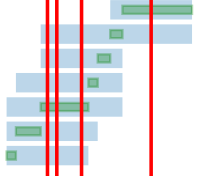
\includegraphics[width=4cm]{Plots/appendix/example.png}};
    % Koordinatensystem
    \draw[line width=0.25mm, ->] (-5,0) -- (-5,5);
    \draw[line width=0.25mm, ->] (-5,0) -- (10,0);
    \node at (10,-0.5) {time};
    \node at (-5.5,3) {rate};
    % Quellen
    \draw[line width=0.5mm, green] (-1,-1) -- (-1,4);
    \fill[pattern = north east lines, pattern color = green, opacity = 0.5,domain=-3:1,variable=\x]
    (-3,0)
    -- plot ({\x},{3.5})
    -- (1,0)
    -- cycle;
    \fill[pattern = north east lines, pattern color = green, opacity = 0.5,domain=-3:1,variable=\x]
    (-3,0)
    -- plot ({\x},{-0.5})
    -- (1,0)
    -- cycle;
    \draw[green] (-3,-0.5) -- (1,-0.5);
    \draw[green] (-3,3.5) -- (1,3.5);
    \draw[green] (-3,-0.5) -- (-3,3.5);
    \draw[green] (1,-0.5) -- (1,3.5);
    \node[green] at (-1,4.5) {$k=1$};

    \draw[line width=0.5mm, orange] (-0.8,-1) -- (-0.8,4);
    \fill[pattern = north east lines, pattern color = orange, opacity = 0.5,domain=-2.8:1.2,variable=\x]
    (-2.8,0)
    -- plot ({\x},{3.5})
    -- (1.2,0)
    -- cycle;
    \fill[pattern = north east lines, pattern color = orange, opacity = 0.5,domain=-2.8:1.2,variable=\x]
    (-2.8,0)
    -- plot ({\x},{-0.5})
    -- (1.2,0)
    -- cycle;
    \draw[orange] (-2.8,-0.5) -- (1.2,-0.5);
    \draw[orange] (-2.8,3.5) -- (1.2,3.5);
    \draw[orange] (-2.8,-0.5) -- (-2.8,3.5);
    \draw[orange] (1.2,-0.5) -- (1.2,3.5);
    \node[orange] at (-0.8,-1.5) {$k=2$};

    \draw[line width=0.5mm, red] (2.5,-1) -- (2.5,4);
    \fill[pattern = north west lines, pattern color = red, opacity = 0.5,domain=0.5:4.5,variable=\x]
    (0.5,0)
    -- plot ({\x},{3.5})
    -- (4.5,0)
    -- cycle;
    \fill[pattern = north west lines, pattern color = red, opacity = 0.5,domain=0.5:4.5,variable=\x]
    (0.5,0)
    -- plot ({\x},{-0.5})
    -- (4.5,0)
    -- cycle;
    \draw[red] (0.5,-0.5) -- (4.5,-0.5);
    \draw[red] (0.5,3.5) -- (4.5,3.5);
    \draw[red] (0.5,-0.5) -- (0.5,3.5);
    \draw[red] (4.5,-0.5) -- (4.5,3.5);
    \node[red] at (2.5,4.5) {$k=3$};

    \draw[line width=0.5mm, blue] (6,-1) -- (6,4);
    \fill[pattern = north east lines, pattern color = blue, opacity = 0.5, domain=4:8,variable=\x]
    (4,0)
    -- plot ({\x},{3.5})
    -- (8,0)
    -- cycle;
    \fill[pattern = north east lines, pattern color = blue, opacity = 0.5,domain=4:8,variable=\x]
    (4,0)
    -- plot ({\x},{-0.5})
    -- (8,0)
    -- cycle;
    \draw[blue] (4,-0.5) -- (8,-0.5);
    \draw[blue] (4,3.5) -- (8,3.5);
    \draw[blue] (4,-0.5) -- (4,3.5);
    \draw[blue] (8,-0.5) -- (8,3.5);
    \node[blue] at (6,4.5) {$k=4$};
    % Samples
    %\draw[line width=0.5mm] (6,-2) -- (6,5);
    %\draw[line width=0.5mm] (0,-2) -- (0,5);
    %\node at (-3,5) {j=1};
    %\node at (3,5) {j=2};
    %\node at (8,5) {j=3};
    % Events
    %\draw[line width=0.5mm,orange] (5,-2) -- (5,1);
    %\draw[line width=0.5mm,orange] (8,-2) -- (8,1);
    %\draw[line width=0.5mm,orange] (3,-2) -- (3,1);
    %\draw[line width=0.5mm,orange] (0.75,-1) -- (0.75,1);
    %\node at (0.9,-1.5) {\quad$0.5$};
    %\node at (3.1,-1.5) {\quad$1$};
    %\node at (5.1,-1.5) {\quad$0$};
    %\node at (8.1,-1.5) {\quad$1$};
    %\node[orange] at (0.75,-1.5) {$i=1$};
    %\node[orange] at (3,-2.5) {i=2};
    %\node[orange] at (5,-2.5) {i=1};
    %\node[orange] at (8,-2.5) {i=4};
    % Nodes
    %\node at (-1,-1.5) {$T_k(t_i)=$};
    %\node[gray] at (-5.8,1.5) {bg-rate};
    % sinus rate
    %\fill [pattern=north east lines,pattern color = blue, domain=2:6, variable=\x]
    %(2, 0)
    %-- plot ({\x}, {sin{(100*\x)}+2})
    %-- (6, 0)
    %-- cycle;
    %\fill [pattern=north east lines,pattern color = red, domain=5:6, variable=\x]
    %(5, 0)
    %-- plot ({\x}, {sin{(100*\x)}+1.5})
    %-- (6, 0)
    %-- cycle;
    %\draw[gray, thick,smooth,domain=0:6 , variable=\x] plot({\x},{0.5*sin{(100*\x)}+2});
    \draw[gray, line width=0.5mm, smooth,domain=-5:0, variable=\x] plot({\x},{0.5*sin{(100*\x)}+1.5});
    \draw[gray, line width=0.5mm, smooth,domain=0:5, variable=\x] plot({\x},{0.5*sin{(100*\x)}+1.5});
    \draw[gray, line width=0.5mm, smooth,domain=5:10, variable=\x] plot({\x},{0.5*sin{(100*\x)}+1.5});
    %\draw[gray, thick,smooth,domain=6:10, variable=\x] plot({\x},{0.5*sin{(100*\x)}+1});
    % intervals
    %\node at (2.5,7.25) {Old method: $\langle\lambda_{B,i=1}\rangle = \langle\lambda_{B,unique}\rangle$};
    %\draw[thick] (-3,7) -- (8,7);
    %\draw[thick] (-3,6.75) -- (-3,7.25);
    %\draw[thick] (8,6.75) -- (8,7.25);
    %\node at (0.75,6.25) {New method: $\langle\lambda_{B,i=1}\rangle = \langle\lambda_{B,\{k=1\cup k=2\}}\rangle$};
    %\draw[thick] (-3,6) -- (4.5,6);
    %\draw[thick] (-3,5.75) -- (-3,6.25);
    %\draw[thick] (4.5,5.75) -- (4.5,6.25);
    %thingie
    %\draw[thick, ->] (-5) -- (10);
    % arrow to picture
    \draw[very thick, ->, color=black] (-5.5,2.5) -- (-7,2.5);
  \end{tikzpicture}}
  \caption{This figure shows a scenario of $\num{4}$ sources $k$ with their time windows (dashed areas). Each unique temporal position translates into a green area on the left, so does a source with a red line. Each green interval is the activation region indicating that an event falling into that region gets compared to an estimated background created in the underlying light blue temporal interval. The scenario therefore generates $\num{7}$ different models. The grey line shows the background rate with its seasonal variations.}
  \label{fig:activation}
\end{figure}
The number of models $\mathcal{B}$ to be calculated in advance can be estimated as,
\begin{equation}
  N_{\text{srcs}} \leq \mathcal{B}\leq 2N_{\text{srcs}}-1, \label{eq:number_of_models}
\end{equation}
with the number of sources $N_{\text{srcs}}$.
So in the worst case scenario this calculation may become about two times slower.
Fortunately, this only affects the spatial PDF and not the energy distribution, as the spatial background depends on the position of the time window due to seasonal variations.
The energy distribution can be extracted from the summation of events and calculated as before.
The temporal PDF is effectively a Heaviside function that attributes the events to the sources weighted by the number of sources they can be attributed to.
With these thoughts in mind, a new injection model needs to be built that injects the right number of background events depending on the temporal position.

To achieve all of the above, the point source software \texttt{tdepps} \cite{tdepps_1} was modified.
The modified version can be found at \cite{tdepps_2}.

However, after the implementation was completed, test results showed unexpected behaviour compared to other software.
The biggest issue are the large values of the test statistics.
A simple example is shown in figure \ref{fig:fail_example}.
Since the correctness of the shape of the test statistic is difficult to assess in the case of a specific time window, in the example the time window is extended over a single complete data set with only one source being investigated.
The behaviour should therefore correspond to a time-integrated search, a $\chi^2$-distribution with only one degree of freedom would be expected, in other words a flat, straight distribution.
However, the modified software still produces too high, signal-like test statistic values, comparable to these of figure \ref{fig:time_dep_sig_sens_ts} in the appendix.
In addition, the behaviour of the \texttt{skylab} software was considered, which is similar to the original behaviour of the unmodified \texttt{tdepps} software.
The \texttt{skylab} result can be seen in figure \ref{fig:skylab}.
\begin{figure}%
    \centering
    \subfloat[\centering Background trials using the reworked \texttt{tdepps} software.]{{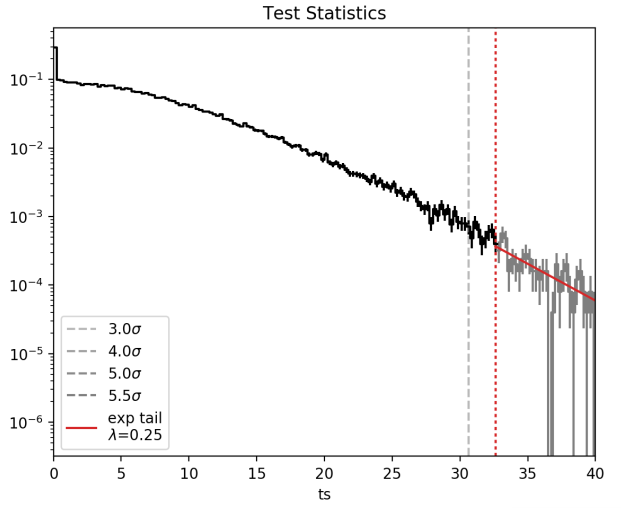
\includegraphics[width=6cm]{Plots/06_tdepps/tdepps_version3_single_bg_pdfs_close.png} }}%
    \qquad
    \subfloat[\centering Background trials using the \texttt{tdepps} software.]{{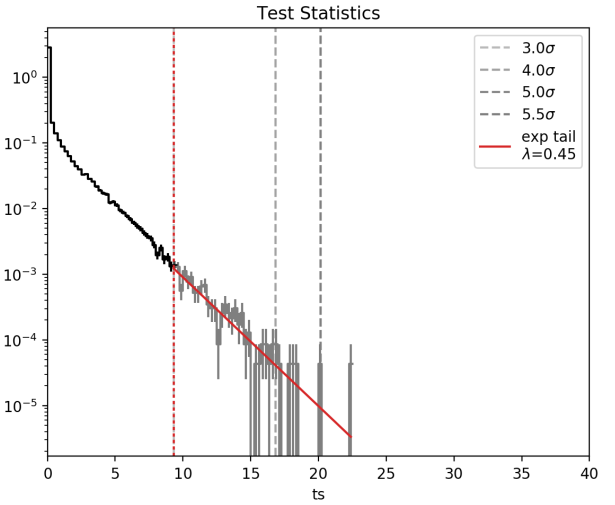
\includegraphics[width=6cm]{Plots/06_tdepps/torben_bg_pdfs_close_real.png} }}%
    \caption{Background trials for $\num{1}$ source with a timewindow expanding over the whole used data set. The y-axis shows the density of trials.}%
    \label{fig:fail_example}%
\end{figure}
\begin{figure}
    \centering
    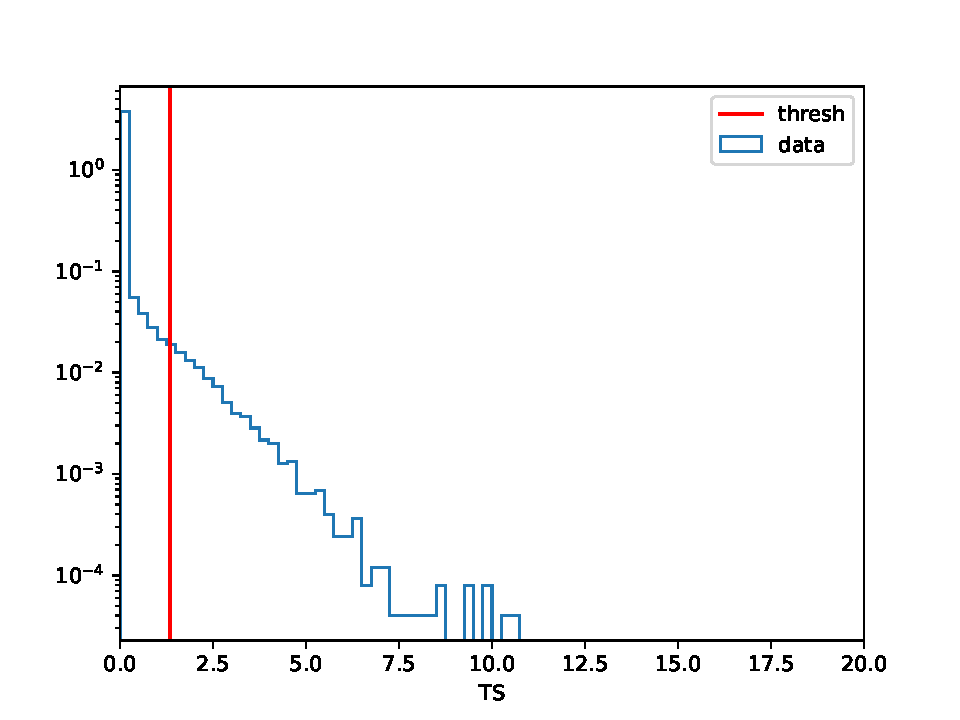
\includegraphics[width=10cm]{Plots/06_tdepps/skylab_bg_pdf_one_source.pdf}
    \caption{Background trials for $\num{1}$ source with a timewindow expanding over the whole used data set using the software \texttt{skylab} version $\num{2.2}$. The y-axis shows the density of trials. The vertical red line indicates the beginning of the straightest possible tail of the statistic determined by various statistical criteria.}
    \label{fig:skylab}
\end{figure}

The main focus of the subsequent research was on the weights that distribute the contribution of the events among the individual sources.
However, this feature works as intended.
Suspicions that this unexpected behaviour could be due to mistakes in the original \texttt{tdepps} software could not be confirmed.
However, as no solution was found to alleviate these problems, the usage of modified \texttt{tdepps} was abandoned.
